% Created by tikzDevice version 0.12.3 on 2020-01-08 13:36:02
% !TEX encoding = UTF-8 Unicode
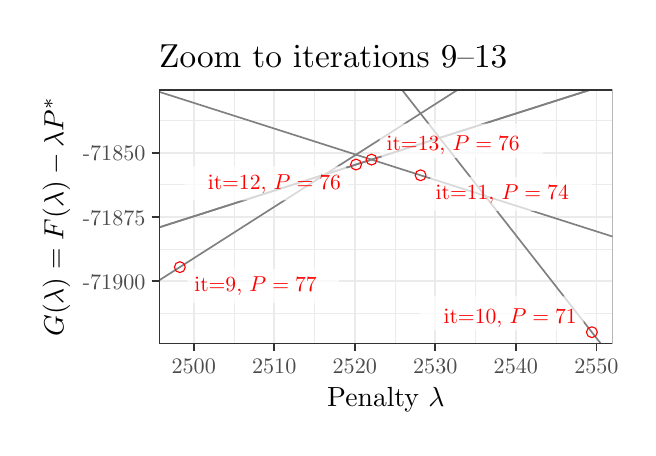
\begin{tikzpicture}[x=1pt,y=1pt]
\definecolor{fillColor}{RGB}{255,255,255}
\path[use as bounding box,fill=fillColor,fill opacity=0.00] (0,0) rectangle (216.81,144.54);
\begin{scope}
\path[clip] (  0.00,  0.00) rectangle (216.81,144.54);
\definecolor{drawColor}{RGB}{255,255,255}
\definecolor{fillColor}{RGB}{255,255,255}

\path[draw=drawColor,line width= 0.6pt,line join=round,line cap=round,fill=fillColor] (  0.00,  0.00) rectangle (216.81,144.54);
\end{scope}
\begin{scope}
\path[clip] ( 47.53, 30.33) rectangle (211.31,122.12);
\definecolor{fillColor}{RGB}{255,255,255}

\path[fill=fillColor] ( 47.53, 30.33) rectangle (211.31,122.12);
\definecolor{drawColor}{gray}{0.92}

\path[draw=drawColor,line width= 0.3pt,line join=round] ( 47.53, 41.31) --
	(211.31, 41.31);

\path[draw=drawColor,line width= 0.3pt,line join=round] ( 47.53, 64.54) --
	(211.31, 64.54);

\path[draw=drawColor,line width= 0.3pt,line join=round] ( 47.53, 87.76) --
	(211.31, 87.76);

\path[draw=drawColor,line width= 0.3pt,line join=round] ( 47.53,110.98) --
	(211.31,110.98);

\path[draw=drawColor,line width= 0.3pt,line join=round] ( 74.54, 30.33) --
	( 74.54,122.12);

\path[draw=drawColor,line width= 0.3pt,line join=round] (103.64, 30.33) --
	(103.64,122.12);

\path[draw=drawColor,line width= 0.3pt,line join=round] (132.75, 30.33) --
	(132.75,122.12);

\path[draw=drawColor,line width= 0.3pt,line join=round] (161.85, 30.33) --
	(161.85,122.12);

\path[draw=drawColor,line width= 0.3pt,line join=round] (190.96, 30.33) --
	(190.96,122.12);

\path[draw=drawColor,line width= 0.6pt,line join=round] ( 47.53, 52.92) --
	(211.31, 52.92);

\path[draw=drawColor,line width= 0.6pt,line join=round] ( 47.53, 76.15) --
	(211.31, 76.15);

\path[draw=drawColor,line width= 0.6pt,line join=round] ( 47.53, 99.37) --
	(211.31, 99.37);

\path[draw=drawColor,line width= 0.6pt,line join=round] ( 59.99, 30.33) --
	( 59.99,122.12);

\path[draw=drawColor,line width= 0.6pt,line join=round] ( 89.09, 30.33) --
	( 89.09,122.12);

\path[draw=drawColor,line width= 0.6pt,line join=round] (118.20, 30.33) --
	(118.20,122.12);

\path[draw=drawColor,line width= 0.6pt,line join=round] (147.30, 30.33) --
	(147.30,122.12);

\path[draw=drawColor,line width= 0.6pt,line join=round] (176.40, 30.33) --
	(176.40,122.12);

\path[draw=drawColor,line width= 0.6pt,line join=round] (205.51, 30.33) --
	(205.51,122.12);
\definecolor{drawColor}{gray}{0.50}

\path[draw=drawColor,line width= 0.6pt,line join=round] ( 47.53, 53.25) -- (190.55,144.54);

\path[draw=drawColor,line width= 0.6pt,line join=round] (117.67,144.54) -- (211.31, 25.00);

\path[draw=drawColor,line width= 0.6pt,line join=round] ( 47.53,121.35) -- (211.31, 69.08);

\path[draw=drawColor,line width= 0.6pt,line join=round] ( 47.53, 72.38) -- (211.31,124.65);

\path[draw=drawColor,line width= 0.6pt,line join=round] ( 47.53, 72.38) -- (211.31,124.65);
\definecolor{fillColor}{RGB}{255,255,255}

\path[fill=fillColor,fill opacity=0.70] ( 59.70, 45.02) --
	(110.50, 45.02) --
	(110.42, 45.02) --
	(110.74, 45.03) --
	(111.05, 45.10) --
	(111.35, 45.21) --
	(111.63, 45.37) --
	(111.88, 45.57) --
	(112.09, 45.81) --
	(112.26, 46.08) --
	(112.38, 46.38) --
	(112.46, 46.69) --
	(112.49, 47.01) --
	(112.49, 47.01) --
	(112.49, 55.39) --
	(112.49, 55.39) --
	(112.46, 55.71) --
	(112.38, 56.02) --
	(112.26, 56.32) --
	(112.09, 56.59) --
	(111.88, 56.83) --
	(111.63, 57.03) --
	(111.35, 57.19) --
	(111.05, 57.30) --
	(110.74, 57.36) --
	(110.50, 57.38) --
	( 59.70, 57.38) --
	( 59.94, 57.36) --
	( 59.62, 57.38) --
	( 59.31, 57.34) --
	( 59.00, 57.25) --
	( 58.71, 57.11) --
	( 58.45, 56.93) --
	( 58.22, 56.71) --
	( 58.02, 56.45) --
	( 57.87, 56.17) --
	( 57.77, 55.87) --
	( 57.72, 55.55) --
	( 57.72, 55.39) --
	( 57.72, 47.01) --
	( 57.72, 47.17) --
	( 57.72, 46.85) --
	( 57.77, 46.53) --
	( 57.87, 46.23) --
	( 58.02, 45.94) --
	( 58.22, 45.69) --
	( 58.45, 45.47) --
	( 58.71, 45.29) --
	( 59.00, 45.15) --
	( 59.31, 45.06) --
	( 59.62, 45.02) --
	cycle;
\end{scope}
\begin{scope}
\path[clip] ( 47.53, 30.33) rectangle (211.31,122.12);
\definecolor{drawColor}{RGB}{255,0,0}

\node[text=drawColor,anchor=base west,inner sep=0pt, outer sep=0pt, scale=  0.78] at ( 60.21, 49.15) {it=9, $P=77$};
\definecolor{fillColor}{RGB}{255,255,255}

\path[fill=fillColor,fill opacity=0.70] (143.88, 35.12) --
	(198.93, 35.12) --
	(198.85, 35.12) --
	(199.17, 35.13) --
	(199.48, 35.20) --
	(199.78, 35.31) --
	(200.06, 35.47) --
	(200.30, 35.67) --
	(200.52, 35.91) --
	(200.69, 36.18) --
	(200.81, 36.48) --
	(200.89, 36.79) --
	(200.91, 37.11) --
	(200.91, 37.11) --
	(200.91, 45.49) --
	(200.91, 45.49) --
	(200.89, 45.81) --
	(200.81, 46.12) --
	(200.69, 46.41) --
	(200.52, 46.69) --
	(200.30, 46.92) --
	(200.06, 47.13) --
	(199.78, 47.29) --
	(199.48, 47.40) --
	(199.17, 47.46) --
	(198.93, 47.48) --
	(143.88, 47.48) --
	(144.12, 47.46) --
	(143.80, 47.48) --
	(143.48, 47.44) --
	(143.18, 47.35) --
	(142.89, 47.21) --
	(142.62, 47.03) --
	(142.39, 46.81) --
	(142.20, 46.55) --
	(142.05, 46.27) --
	(141.95, 45.97) --
	(141.90, 45.65) --
	(141.89, 45.49) --
	(141.89, 37.11) --
	(141.90, 37.27) --
	(141.90, 36.95) --
	(141.95, 36.63) --
	(142.05, 36.33) --
	(142.20, 36.04) --
	(142.39, 35.79) --
	(142.62, 35.57) --
	(142.89, 35.38) --
	(143.18, 35.25) --
	(143.48, 35.16) --
	(143.80, 35.12) --
	cycle;
\end{scope}
\begin{scope}
\path[clip] ( 47.53, 30.33) rectangle (211.31,122.12);
\definecolor{drawColor}{RGB}{255,0,0}

\node[text=drawColor,anchor=base east,inner sep=0pt, outer sep=0pt, scale=  0.78] at (198.42, 37.61) {it=10, $P=71$};
\definecolor{fillColor}{RGB}{255,255,255}

\path[fill=fillColor,fill opacity=0.70] (146.90, 78.23) --
	(201.95, 78.23) --
	(201.87, 78.23) --
	(202.19, 78.25) --
	(202.50, 78.31) --
	(202.80, 78.42) --
	(203.08, 78.58) --
	(203.33, 78.79) --
	(203.54, 79.03) --
	(203.71, 79.30) --
	(203.83, 79.59) --
	(203.91, 79.90) --
	(203.94, 80.22) --
	(203.94, 80.22) --
	(203.94, 88.61) --
	(203.94, 88.61) --
	(203.91, 88.92) --
	(203.83, 89.23) --
	(203.71, 89.53) --
	(203.54, 89.80) --
	(203.33, 90.04) --
	(203.08, 90.24) --
	(202.80, 90.40) --
	(202.50, 90.51) --
	(202.19, 90.58) --
	(201.95, 90.59) --
	(146.90, 90.59) --
	(147.14, 90.58) --
	(146.82, 90.59) --
	(146.51, 90.55) --
	(146.20, 90.46) --
	(145.91, 90.33) --
	(145.65, 90.14) --
	(145.42, 89.92) --
	(145.22, 89.67) --
	(145.08, 89.38) --
	(144.97, 89.08) --
	(144.92, 88.77) --
	(144.92, 88.61) --
	(144.92, 80.22) --
	(144.92, 80.38) --
	(144.92, 80.06) --
	(144.97, 79.74) --
	(145.08, 79.44) --
	(145.22, 79.16) --
	(145.42, 78.90) --
	(145.65, 78.68) --
	(145.91, 78.50) --
	(146.20, 78.36) --
	(146.51, 78.27) --
	(146.82, 78.23) --
	cycle;
\end{scope}
\begin{scope}
\path[clip] ( 47.53, 30.33) rectangle (211.31,122.12);
\definecolor{drawColor}{RGB}{255,0,0}

\node[text=drawColor,anchor=base west,inner sep=0pt, outer sep=0pt, scale=  0.78] at (147.41, 82.36) {it=11, $P=74$};
\definecolor{fillColor}{RGB}{255,255,255}

\path[fill=fillColor,fill opacity=0.70] ( 58.68, 82.10) --
	(113.72, 82.10) --
	(113.64, 82.10) --
	(113.96, 82.12) --
	(114.28, 82.18) --
	(114.57, 82.29) --
	(114.85, 82.45) --
	(115.10, 82.65) --
	(115.31, 82.89) --
	(115.48, 83.16) --
	(115.61, 83.46) --
	(115.68, 83.77) --
	(115.71, 84.09) --
	(115.71, 84.09) --
	(115.71, 92.47) --
	(115.71, 92.47) --
	(115.68, 92.79) --
	(115.61, 93.10) --
	(115.48, 93.40) --
	(115.31, 93.67) --
	(115.10, 93.91) --
	(114.85, 94.11) --
	(114.57, 94.27) --
	(114.28, 94.38) --
	(113.96, 94.45) --
	(113.72, 94.46) --
	( 58.68, 94.46) --
	( 58.92, 94.45) --
	( 58.60, 94.46) --
	( 58.28, 94.42) --
	( 57.97, 94.33) --
	( 57.68, 94.19) --
	( 57.42, 94.01) --
	( 57.19, 93.79) --
	( 57.00, 93.54) --
	( 56.85, 93.25) --
	( 56.75, 92.95) --
	( 56.70, 92.63) --
	( 56.69, 92.47) --
	( 56.69, 84.09) --
	( 56.70, 84.25) --
	( 56.70, 83.93) --
	( 56.75, 83.61) --
	( 56.85, 83.31) --
	( 57.00, 83.03) --
	( 57.19, 82.77) --
	( 57.42, 82.55) --
	( 57.68, 82.37) --
	( 57.97, 82.23) --
	( 58.28, 82.14) --
	( 58.60, 82.10) --
	cycle;
\end{scope}
\begin{scope}
\path[clip] ( 47.53, 30.33) rectangle (211.31,122.12);
\definecolor{drawColor}{RGB}{255,0,0}

\node[text=drawColor,anchor=base east,inner sep=0pt, outer sep=0pt, scale=  0.78] at (113.21, 86.23) {it=12, $P=76$};
\definecolor{fillColor}{RGB}{255,255,255}

\path[fill=fillColor,fill opacity=0.70] (129.19, 97.48) --
	(184.24, 97.48) --
	(184.16, 97.48) --
	(184.48, 97.50) --
	(184.79, 97.56) --
	(185.09, 97.67) --
	(185.37, 97.83) --
	(185.61, 98.04) --
	(185.83, 98.28) --
	(186.00, 98.55) --
	(186.12, 98.84) --
	(186.20, 99.15) --
	(186.22, 99.47) --
	(186.22, 99.47) --
	(186.22,107.86) --
	(186.22,107.86) --
	(186.20,108.17) --
	(186.12,108.48) --
	(186.00,108.78) --
	(185.83,109.05) --
	(185.61,109.29) --
	(185.37,109.49) --
	(185.09,109.65) --
	(184.79,109.76) --
	(184.48,109.83) --
	(184.24,109.84) --
	(129.19,109.84) --
	(129.43,109.83) --
	(129.11,109.84) --
	(128.79,109.80) --
	(128.49,109.71) --
	(128.20,109.58) --
	(127.94,109.39) --
	(127.70,109.17) --
	(127.51,108.92) --
	(127.36,108.63) --
	(127.26,108.33) --
	(127.21,108.01) --
	(127.20,107.86) --
	(127.20, 99.47) --
	(127.21, 99.63) --
	(127.21, 99.31) --
	(127.26, 98.99) --
	(127.36, 98.69) --
	(127.51, 98.41) --
	(127.70, 98.15) --
	(127.94, 97.93) --
	(128.20, 97.75) --
	(128.49, 97.61) --
	(128.79, 97.52) --
	(129.11, 97.48) --
	cycle;
\end{scope}
\begin{scope}
\path[clip] ( 47.53, 30.33) rectangle (211.31,122.12);
\definecolor{drawColor}{RGB}{255,0,0}

\node[text=drawColor,anchor=base west,inner sep=0pt, outer sep=0pt, scale=  0.78] at (129.70, 99.98) {it=13, $P=76$};

\path[draw=drawColor,line width= 0.4pt,line join=round,line cap=round] ( 54.98, 58.00) circle (  1.96);

\path[draw=drawColor,line width= 0.4pt,line join=round,line cap=round] (203.87, 34.50) circle (  1.96);

\path[draw=drawColor,line width= 0.4pt,line join=round,line cap=round] (141.97, 91.21) circle (  1.96);

\path[draw=drawColor,line width= 0.4pt,line join=round,line cap=round] (118.66, 95.08) circle (  1.96);

\path[draw=drawColor,line width= 0.4pt,line join=round,line cap=round] (124.25, 96.86) circle (  1.96);
\definecolor{drawColor}{gray}{0.20}

\path[draw=drawColor,line width= 0.6pt,line join=round,line cap=round] ( 47.53, 30.33) rectangle (211.31,122.12);
\end{scope}
\begin{scope}
\path[clip] (  0.00,  0.00) rectangle (216.81,144.54);
\definecolor{drawColor}{gray}{0.30}

\node[text=drawColor,anchor=base east,inner sep=0pt, outer sep=0pt, scale=  0.80] at ( 42.58, 49.97) {-71900};

\node[text=drawColor,anchor=base east,inner sep=0pt, outer sep=0pt, scale=  0.80] at ( 42.58, 73.19) {-71875};

\node[text=drawColor,anchor=base east,inner sep=0pt, outer sep=0pt, scale=  0.80] at ( 42.58, 96.41) {-71850};
\end{scope}
\begin{scope}
\path[clip] (  0.00,  0.00) rectangle (216.81,144.54);
\definecolor{drawColor}{gray}{0.20}

\path[draw=drawColor,line width= 0.6pt,line join=round] ( 44.78, 52.92) --
	( 47.53, 52.92);

\path[draw=drawColor,line width= 0.6pt,line join=round] ( 44.78, 76.15) --
	( 47.53, 76.15);

\path[draw=drawColor,line width= 0.6pt,line join=round] ( 44.78, 99.37) --
	( 47.53, 99.37);
\end{scope}
\begin{scope}
\path[clip] (  0.00,  0.00) rectangle (216.81,144.54);
\definecolor{drawColor}{gray}{0.20}

\path[draw=drawColor,line width= 0.6pt,line join=round] ( 59.99, 27.58) --
	( 59.99, 30.33);

\path[draw=drawColor,line width= 0.6pt,line join=round] ( 89.09, 27.58) --
	( 89.09, 30.33);

\path[draw=drawColor,line width= 0.6pt,line join=round] (118.20, 27.58) --
	(118.20, 30.33);

\path[draw=drawColor,line width= 0.6pt,line join=round] (147.30, 27.58) --
	(147.30, 30.33);

\path[draw=drawColor,line width= 0.6pt,line join=round] (176.40, 27.58) --
	(176.40, 30.33);

\path[draw=drawColor,line width= 0.6pt,line join=round] (205.51, 27.58) --
	(205.51, 30.33);
\end{scope}
\begin{scope}
\path[clip] (  0.00,  0.00) rectangle (216.81,144.54);
\definecolor{drawColor}{gray}{0.30}

\node[text=drawColor,anchor=base,inner sep=0pt, outer sep=0pt, scale=  0.80] at ( 59.99, 19.46) {2500};

\node[text=drawColor,anchor=base,inner sep=0pt, outer sep=0pt, scale=  0.80] at ( 89.09, 19.46) {2510};

\node[text=drawColor,anchor=base,inner sep=0pt, outer sep=0pt, scale=  0.80] at (118.20, 19.46) {2520};

\node[text=drawColor,anchor=base,inner sep=0pt, outer sep=0pt, scale=  0.80] at (147.30, 19.46) {2530};

\node[text=drawColor,anchor=base,inner sep=0pt, outer sep=0pt, scale=  0.80] at (176.40, 19.46) {2540};

\node[text=drawColor,anchor=base,inner sep=0pt, outer sep=0pt, scale=  0.80] at (205.51, 19.46) {2550};
\end{scope}
\begin{scope}
\path[clip] (  0.00,  0.00) rectangle (216.81,144.54);
\definecolor{drawColor}{RGB}{0,0,0}

\node[text=drawColor,anchor=base,inner sep=0pt, outer sep=0pt, scale=  1.00] at (129.42,  7.62) {Penalty $\lambda$};
\end{scope}
\begin{scope}
\path[clip] (  0.00,  0.00) rectangle (216.81,144.54);
\definecolor{drawColor}{RGB}{0,0,0}

\node[text=drawColor,rotate= 90.00,anchor=base,inner sep=0pt, outer sep=0pt, scale=  1.00] at ( 12.89, 76.22) {$G(\lambda)=F(\lambda)-\lambda P^*$};
\end{scope}
\begin{scope}
\path[clip] (  0.00,  0.00) rectangle (216.81,144.54);
\definecolor{drawColor}{RGB}{0,0,0}

\node[text=drawColor,anchor=base west,inner sep=0pt, outer sep=0pt, scale=  1.20] at ( 47.53,130.17) {Zoom to iterations 9--13};
\end{scope}
\end{tikzpicture}
